\documentclass[FIPLY_base.tex]{subfiles}

\author{Andreas Denkmayr}
\date{12. März 2016}

\begin{document}
\section{NavigationDrawer}
Der NavigationDrawer ist ein Menü, das die wichtigsten Navigationsoptionen am linken Bildschirmrand darstellt.
Diese Leiste ist meistens versteckt und wird angezeigt sobald der Benutzer mit dem Finger vom linken Rand des Bildschirms in Richtung Bildschirmmitte streicht oder auf das NavigationDrawerIcon klickt.
Erneutes Klicken auf dieses Icon oder Streichen nach links versteckt den NavigationDrawer. \newline
[\citeauthor{bNavDrawer} \cite{bNavDrawer}, \citeauthor{bNavDrawerRT} \cite{bNavDrawerRT}, Android Developers \cite{adNavDrawer}]
\ \\
\begin{figure}[h]
	\begin{subfigure}[b]{0.3\textwidth}
	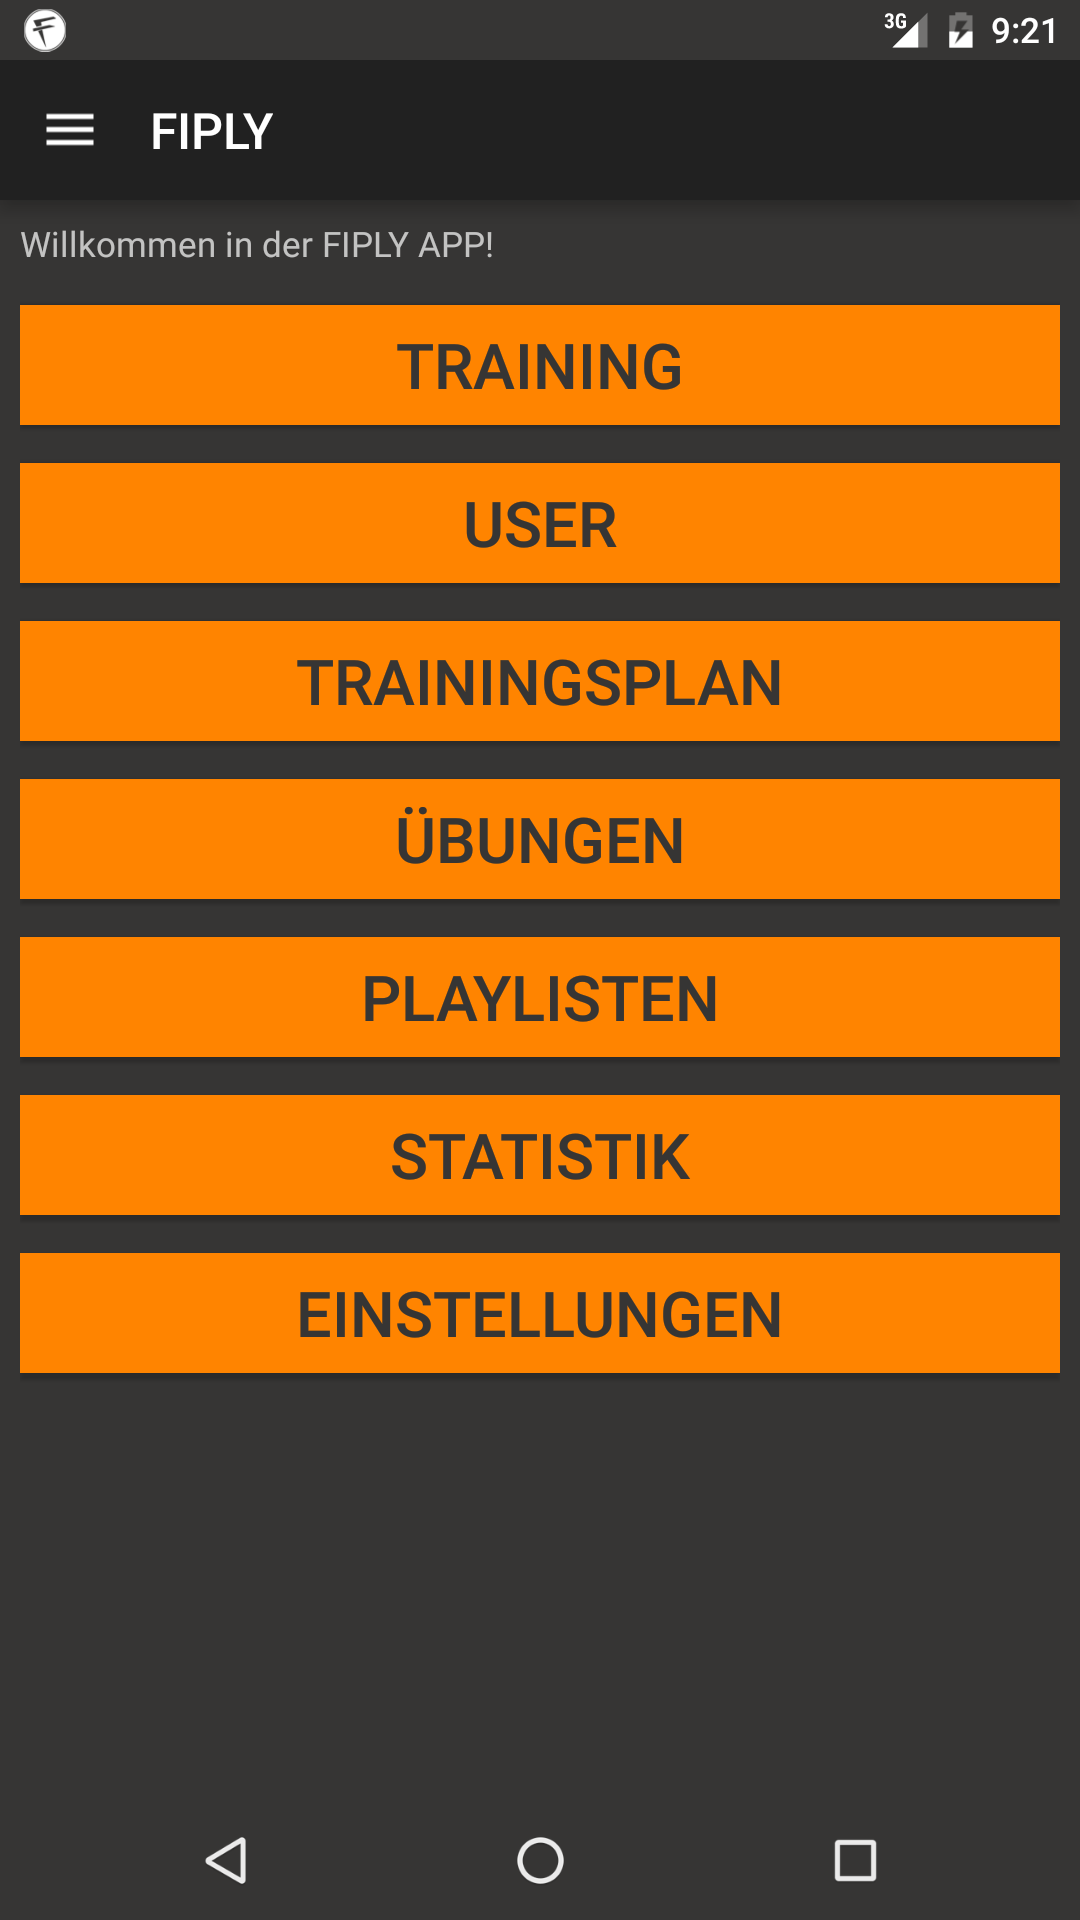
\includegraphics[scale=0.15]{img/NavDrawerClosed}
	\end{subfigure}
	\hfil
	\begin{subfigure}[b]{0.3\textwidth}
	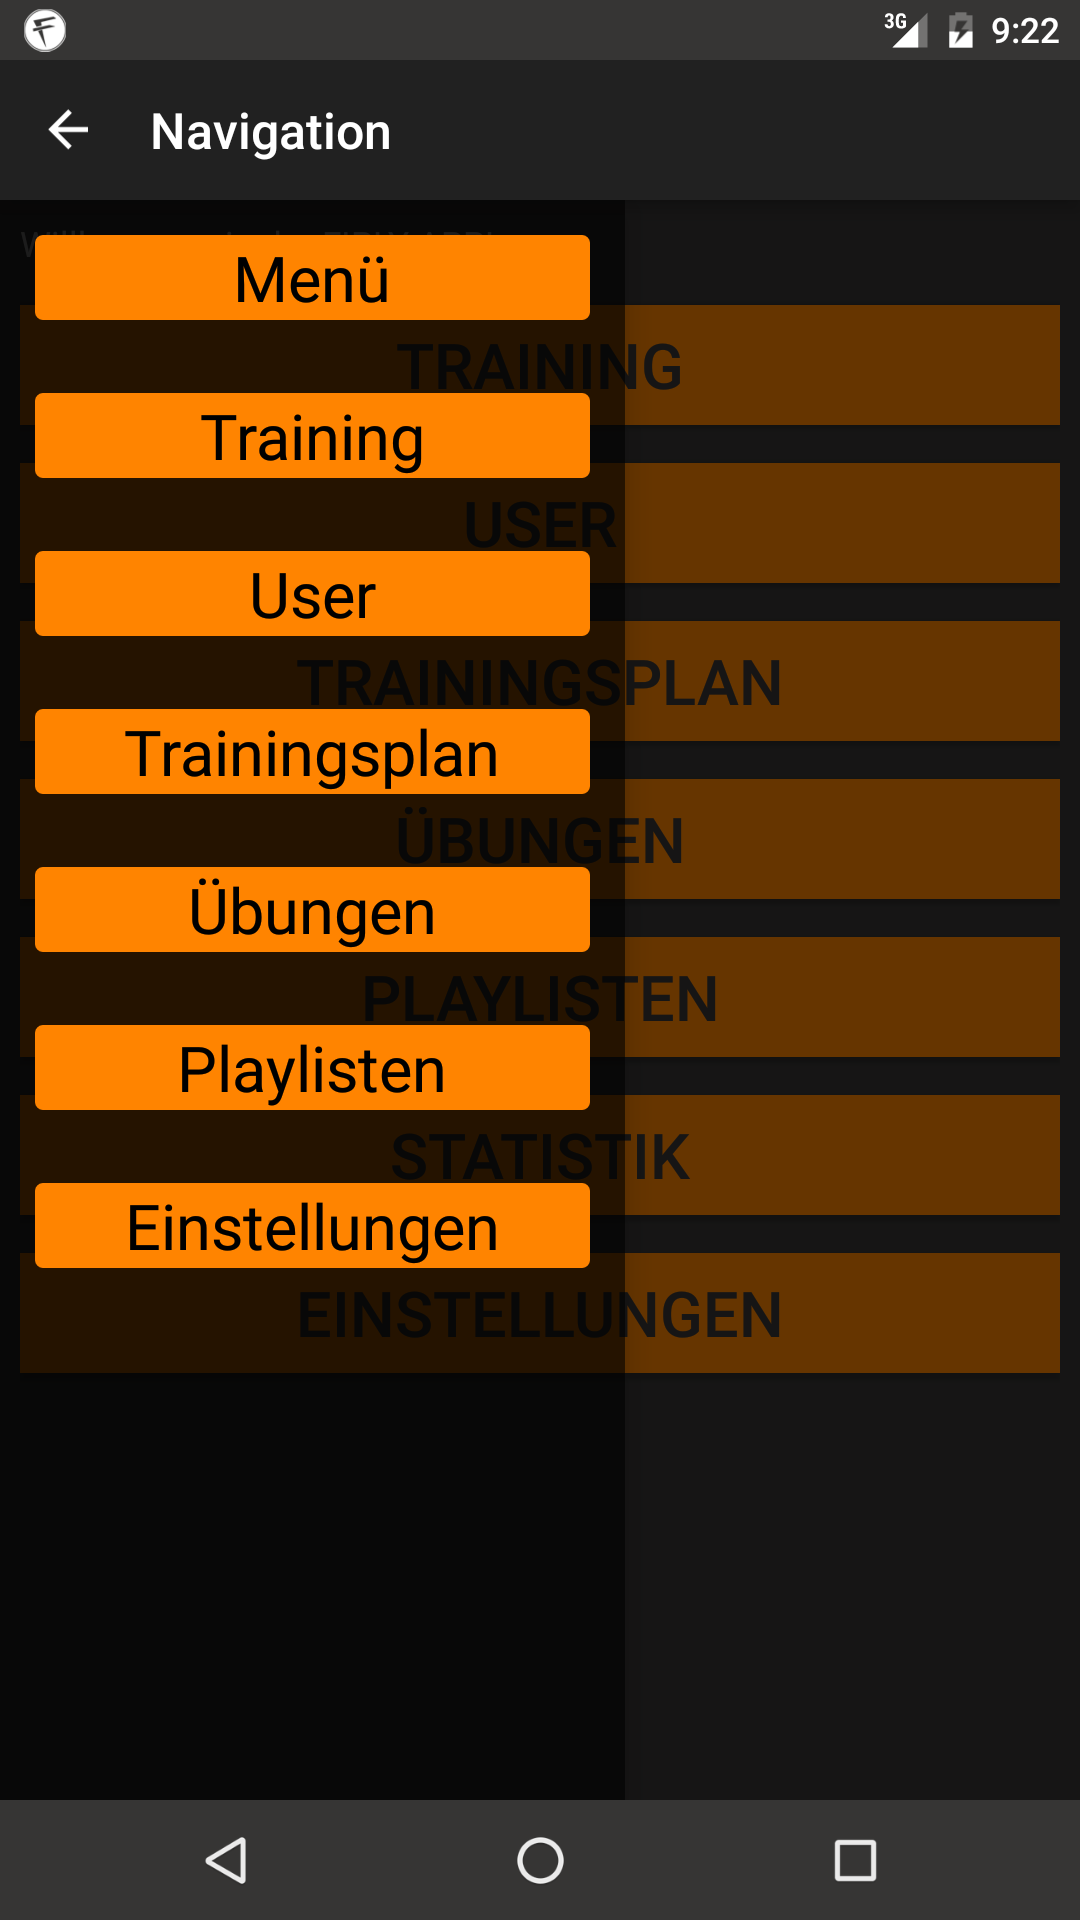
\includegraphics[scale=0.15]{img/NavDrawerOpened}
	\end{subfigure}
	\caption{Links wird der NavigationDrawer versteckt. Rechts ist der NavigationDrawer geöffnet.}
\end{figure}

\newpage
\begin{lstlisting}
<android.support.v4.widget.DrawerLayout
	xmlns:android="http://schemas.android.com/apk/res/android"
	xmlns:tools="http://schemas.android.com/tools"
	android:id="@+id/drawer_layout"
	android:layout_width="match_parent"
	android:layout_height="match_parent"
	tools:context="htl_leonding.fiplyteam.fiply.menu.MainActivity">

	<FrameLayout
		android:id="@+id/fraPlace"
		android:layout_width="match_parent"
		android:layout_height="match_parent" />

	<ListView
		android:id="@+id/navlist"
		android:layout_width="250dp"
		android:layout_height="match_parent"
		android:layout_gravity="start"
		android:background="@color/darkNavigationBackground"
		android:divider="@color/darkNavigationDivider"
		android:dividerHeight="1dp" />

</android.support.v4.widget.DrawerLayout>
\end{lstlisting}
\ \\
Um einen NavigationDrawer zu einer App hinzuzufügen wird ein DrawerLayout als Root-View in dem layout XML file einer Activity deklariert. 
Eine Root-View beinhaltet alle anderen Views der App. 
In diesem DrawerLayout wird anschließend eine View angelegt, die dazu verwendet wird den Hauptinhalt der App darzustellen.
Dabei ist zu Beachten, dass das die View die alle Elemente in sich trägt als erstes Kind des DrawerLayouts deklariert wird.
Da diese View den ganzen Bildschirm befüllen soll müssen die Höhe und die Breite auf ''match\_parent'' gestellt werden.
\ \\
Zusätzlich wird eine weitere View hinzugefügt, die die Elemente des NavigationDrawers in sich trägt. 
Diese muss das Attribut layout\_gravity überschreiben. 
Um right-to-left Sprachen zu unterstützen, soll ''start'' anstatt von ''left'' dafür spezifiziert werden. 
Die Höhe soll die Länge des ganzen Bildschirms umfassen, die Breite wird in Density-independent Pixels definiert und sollte 320dp nicht überschreiten da der Benutzer immer Teile des Hauptinhalts sehen soll. 

\ \\
In dieser Arbeit wird für den Hauptinhalt das FrameLayout fraPlace verwendet. 
Dieses Layout dient als Container für Fragments, die die einzelnen Ansichten der App darstellen.
Die Elemente des NavigationDrawers werden in der ListView navlist definiert.

\newpage
\begin{lstlisting}
public class MainActivity extends AppCompatActivity {
	ListView mDrawerList;
	ArrayAdapter<String> mAdapter;
	DrawerLayout mDrawerLayout;
	String[] navArray = new String[7];
	
	@Override
	protected void onCreate(Bundle savedInstanceState) {
		super.onCreate(savedInstanceState);
		setContentView(R.layout.activity_main);
		
		mDrawerList = (ListView) findViewById(R.id.navlist);
		mDrawerLayout = (DrawerLayout) findViewById(
			R.id.drawer_layout);
		navArray = res.getStringArray(R.array.navigationArray);

		mDrawerList.setOnItemClickListener(new AdapterView
			.OnItemClickListener() {
			
			@Override
			public void onItemClick(AdapterView<?> parent, View view, 
				int position, long id) {		
				displayView(position);
			}
		});
	
		mAdapter = new ArrayAdapter<>(this, R.layout.navigation_list, 
			R.id.navlist_content, navArray);
		mDrawerList.setAdapter(mAdapter)
			}
}
\end{lstlisting}
\ \\
Das ist der minimale Code, um einen funktionierenden NavigationDrawer zu erstellen.
Will man das Design und Verhalten des Icons, zum Öffnen des NavigationDrawers, ändern, ist noch etwas Code nötig.
Dieser Code wird ebenfalls im onCreate der Activity, die einen NavigationDrawer erhalten soll, ausgeführt.
\ \\
\begin{lstlisting}
mDrawerToggle = new ActionBarDrawerToggle(this, mDrawerLayout,
	R.string.drawer_open, R.string.drawer_close) {
	...
};
mDrawerToggle.setDrawerIndicatorEnabled(true);
mDrawerLayout.addDrawerListener(mDrawerToggle);
getSupportActionBar().setDisplayHomeAsUpEnabled(true);
getSupportActionBar().setHomeButtonEnabled(true);
\end{lstlisting}
\end{document}
